\chapter{Evaluation and experiments}
\section{Single Quadrotor Control with Payload}
\begin{figure}[ht]
    \centering
    \begin{subfigure}[b]{0.49\textwidth}
        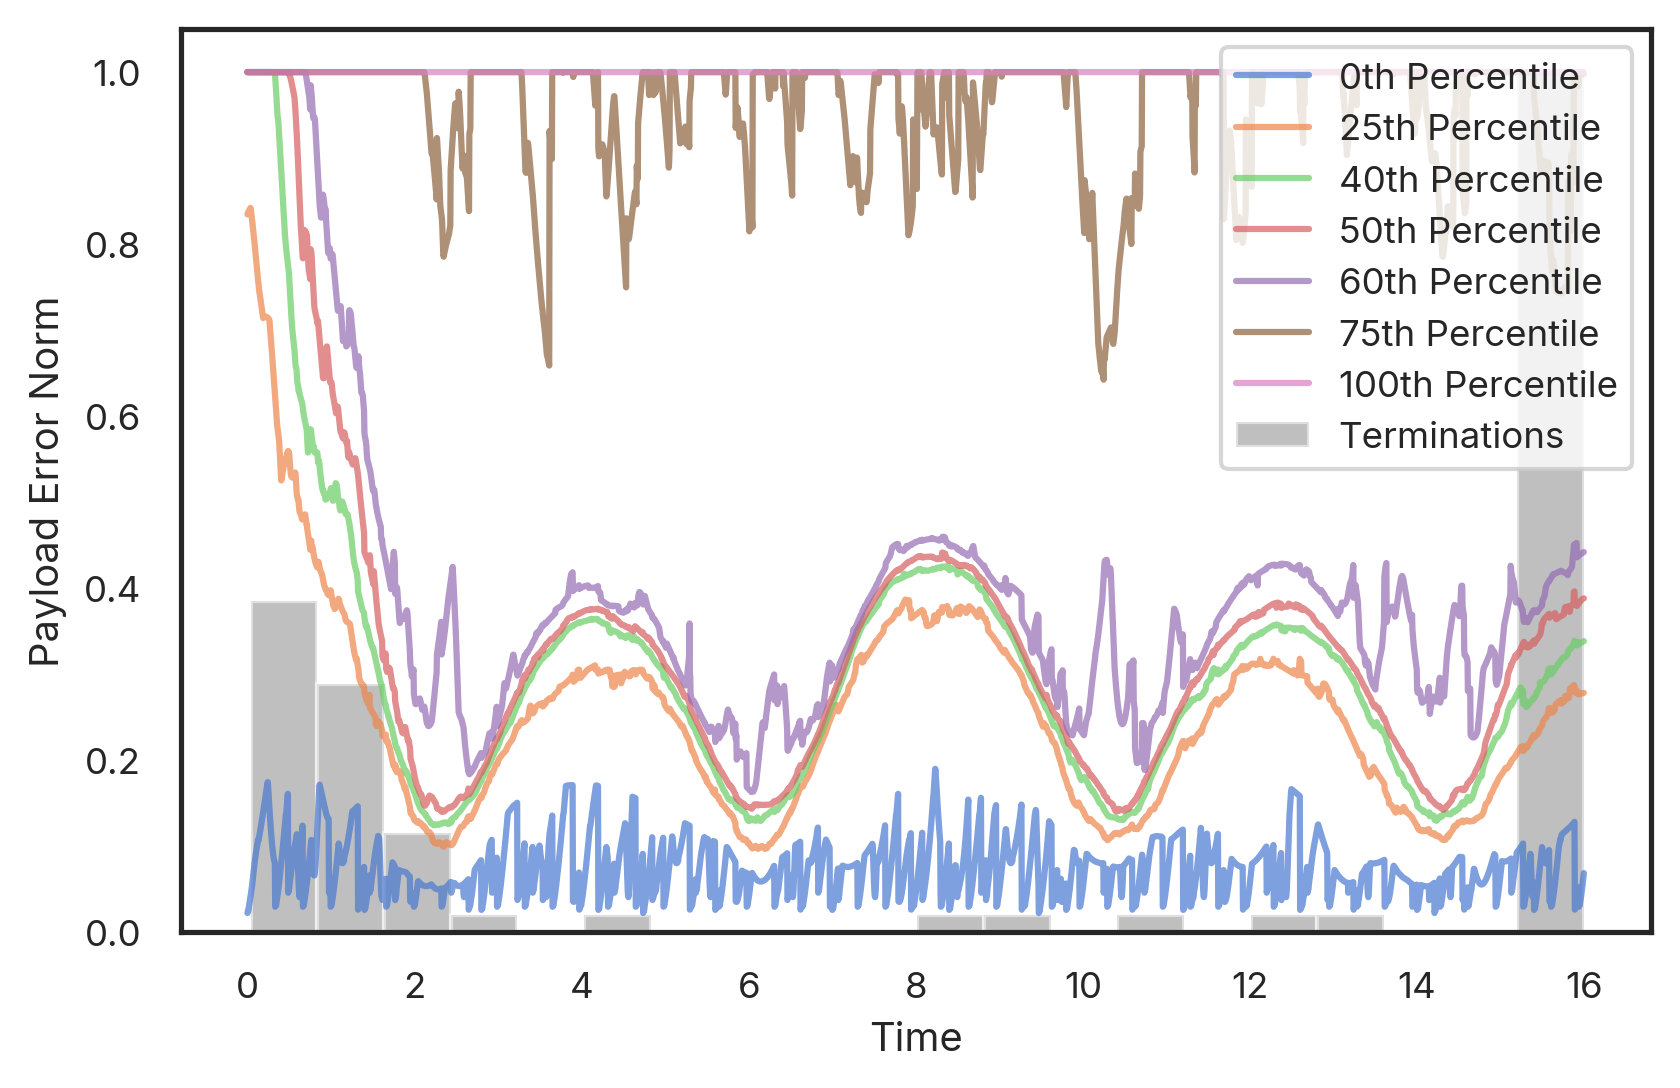
\includegraphics[width=\textwidth]{experiments/payload_error_over_time.png}
        \caption{Error over time for a single quadrotor carrying a payload evaluated over 1000 rollouts. The quadrotor is able to recover from harsh disturbances and track a desired position.}
        \label{fig:payload_error_over_time}
    \end{subfigure}
    \hfill
    \begin{subfigure}[b]{0.49\textwidth}
        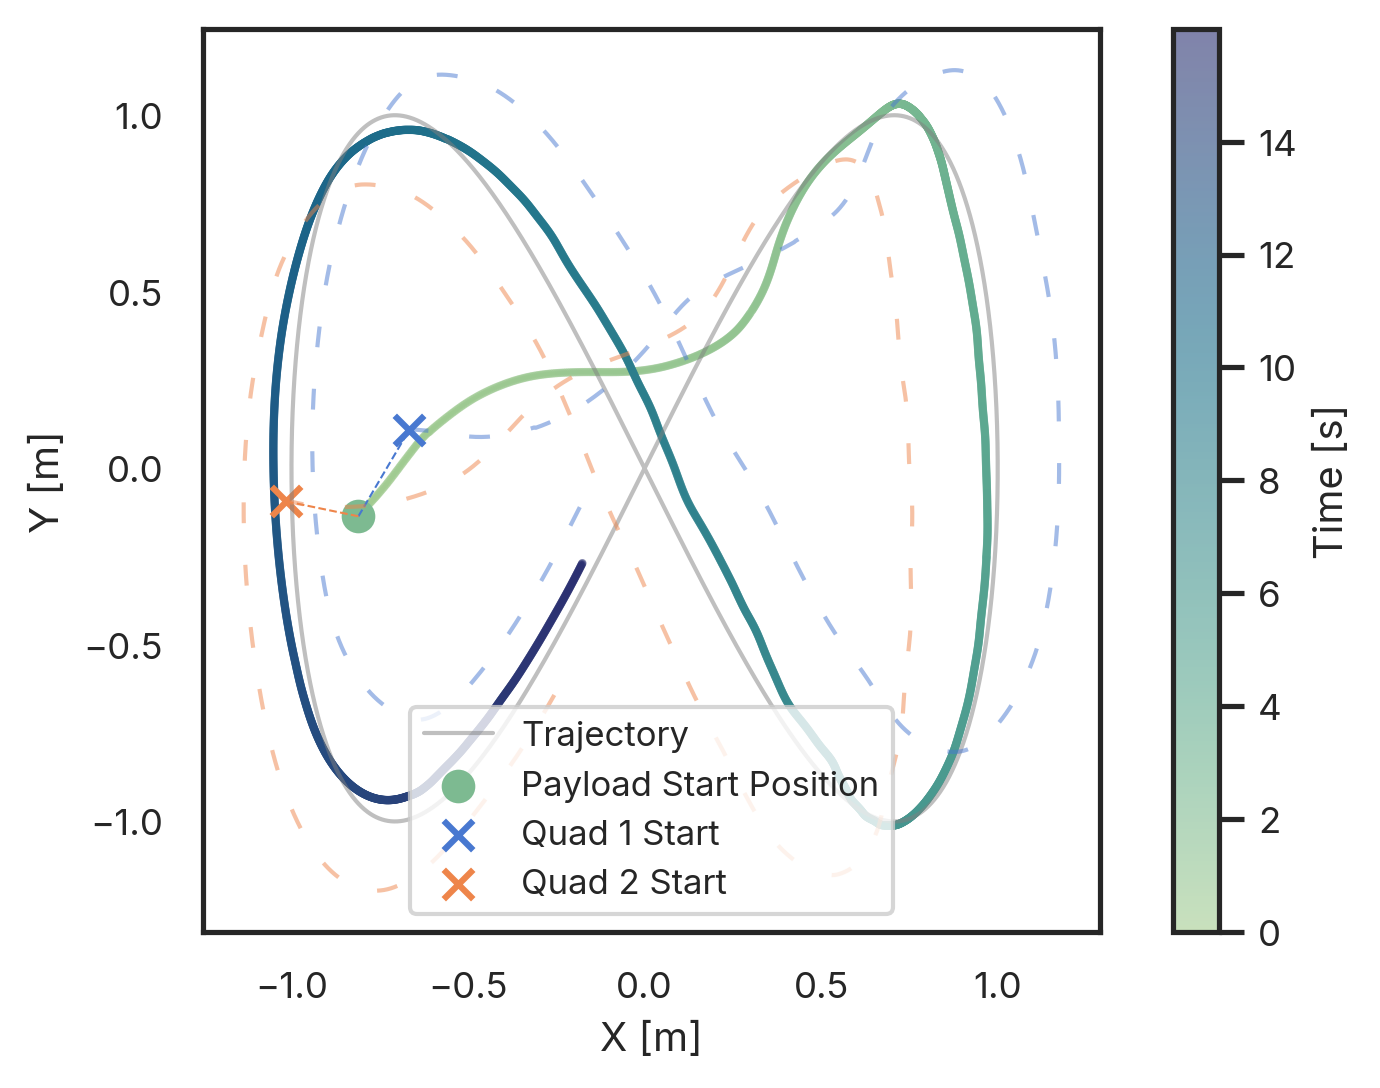
\includegraphics[width=\textwidth]{experiments/payload_position_xy.png}
        \caption{Position over time for a single quadrotor carrying a payload tracking a figure eight trajectory.}
        \label{fig:payload_position_xy}
    \end{subfigure}
    \caption{Single quadrotor control with payload: (a) error over time, (b) position tracking on a figure-eight.}
    \label{fig:single_quad_payload_subfigs}
\end{figure}
\begin{itemize}
    \item Recover from harsh and track position
    \item Follow trajectory
    \item Follow trajectory with disturbance


\end{itemize}

\section{Multi Quadrotor Control with Payload}
\begin{figure}[ht]
    \centering
    % Two quadrotors
    \begin{subfigure}[b]{0.49\textwidth}
        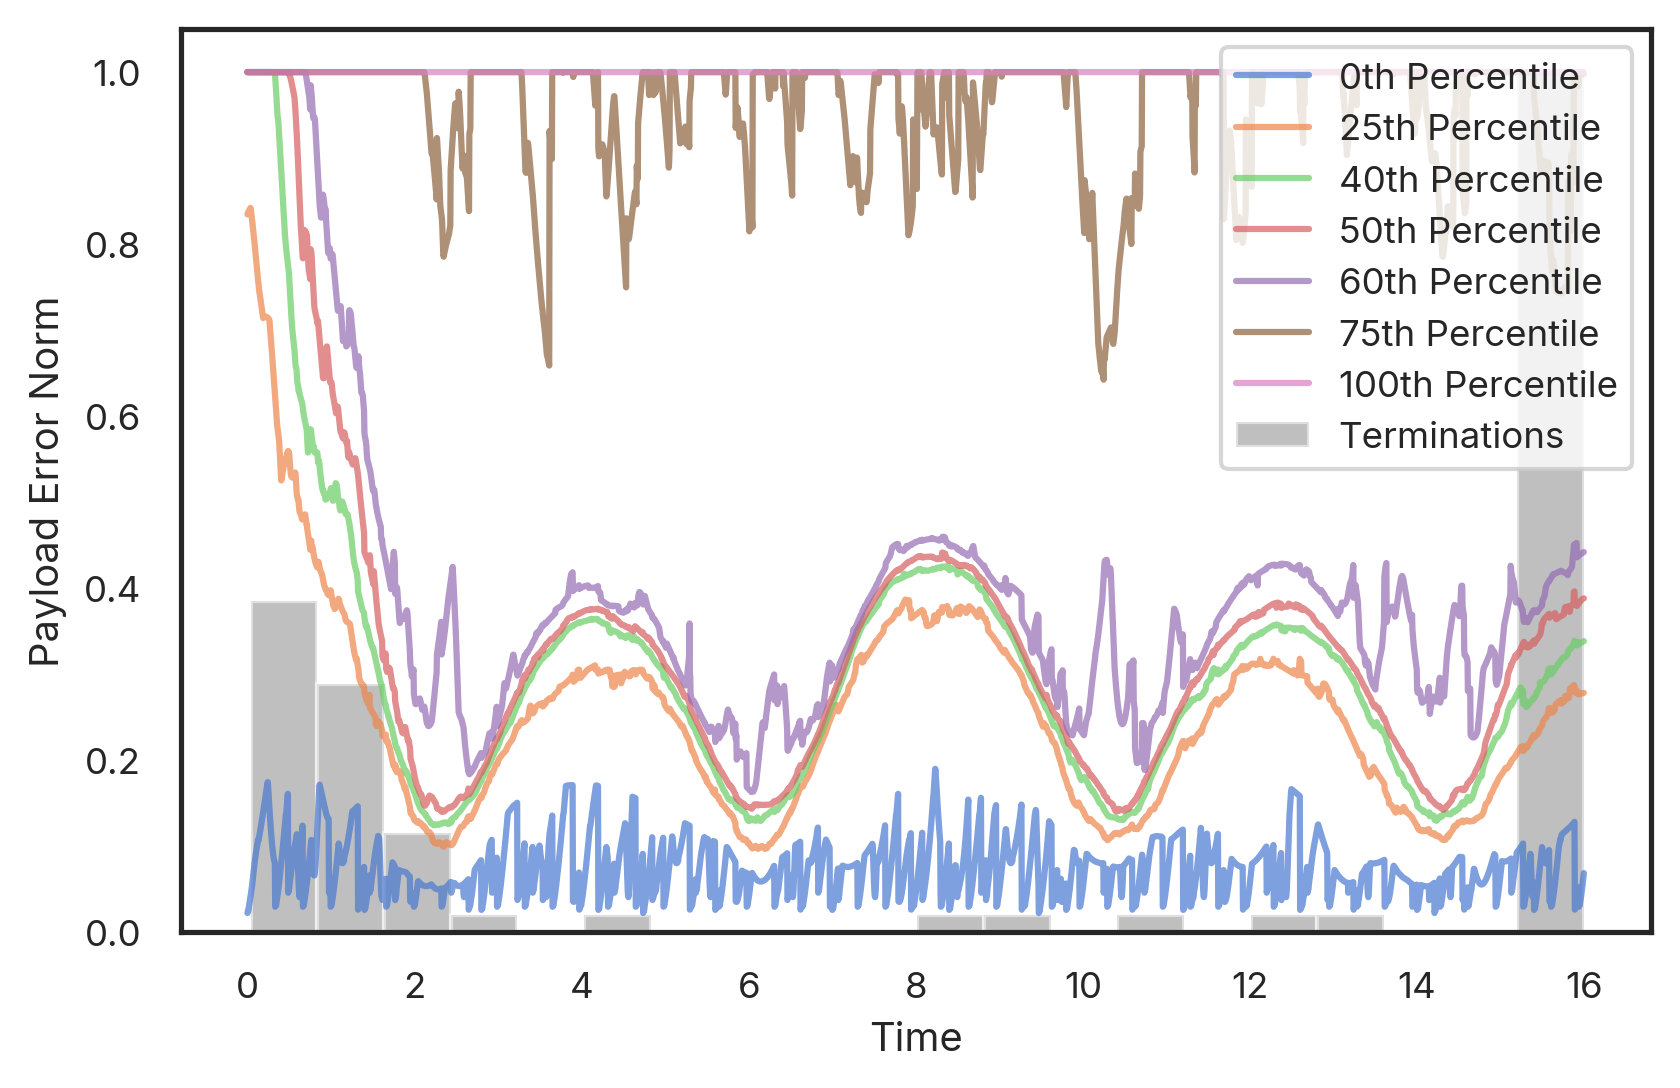
\includegraphics[width=\textwidth]{experiments/payload_error_over_time.png}
        \caption{Error over time for 2 quadrotors with payload (1000 rollouts).}
        \label{fig:payload_error_2quads}
    \end{subfigure}
    \hfill
    \begin{subfigure}[b]{0.49\textwidth}
        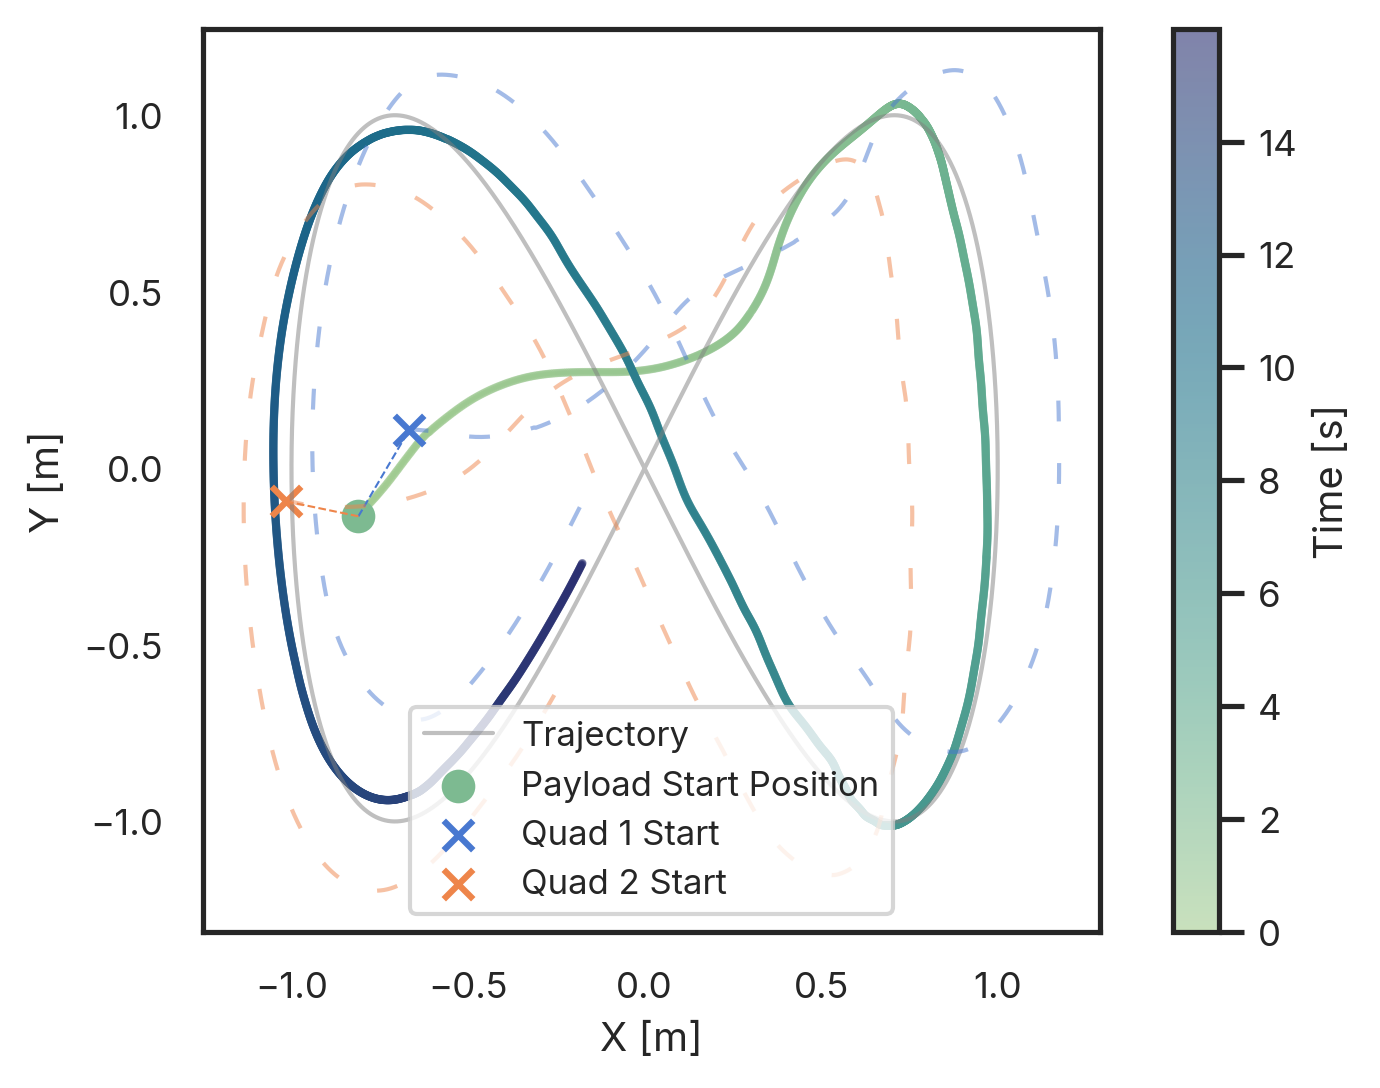
\includegraphics[width=\textwidth]{experiments/payload_position_xy.png}
        \caption{Position tracking for 2 quadrotors on figure-eight.}
        \label{fig:payload_position_2quads}
    \end{subfigure}

    \vspace{1em}

    % Three quadrotors
    \begin{subfigure}[b]{0.49\textwidth}
        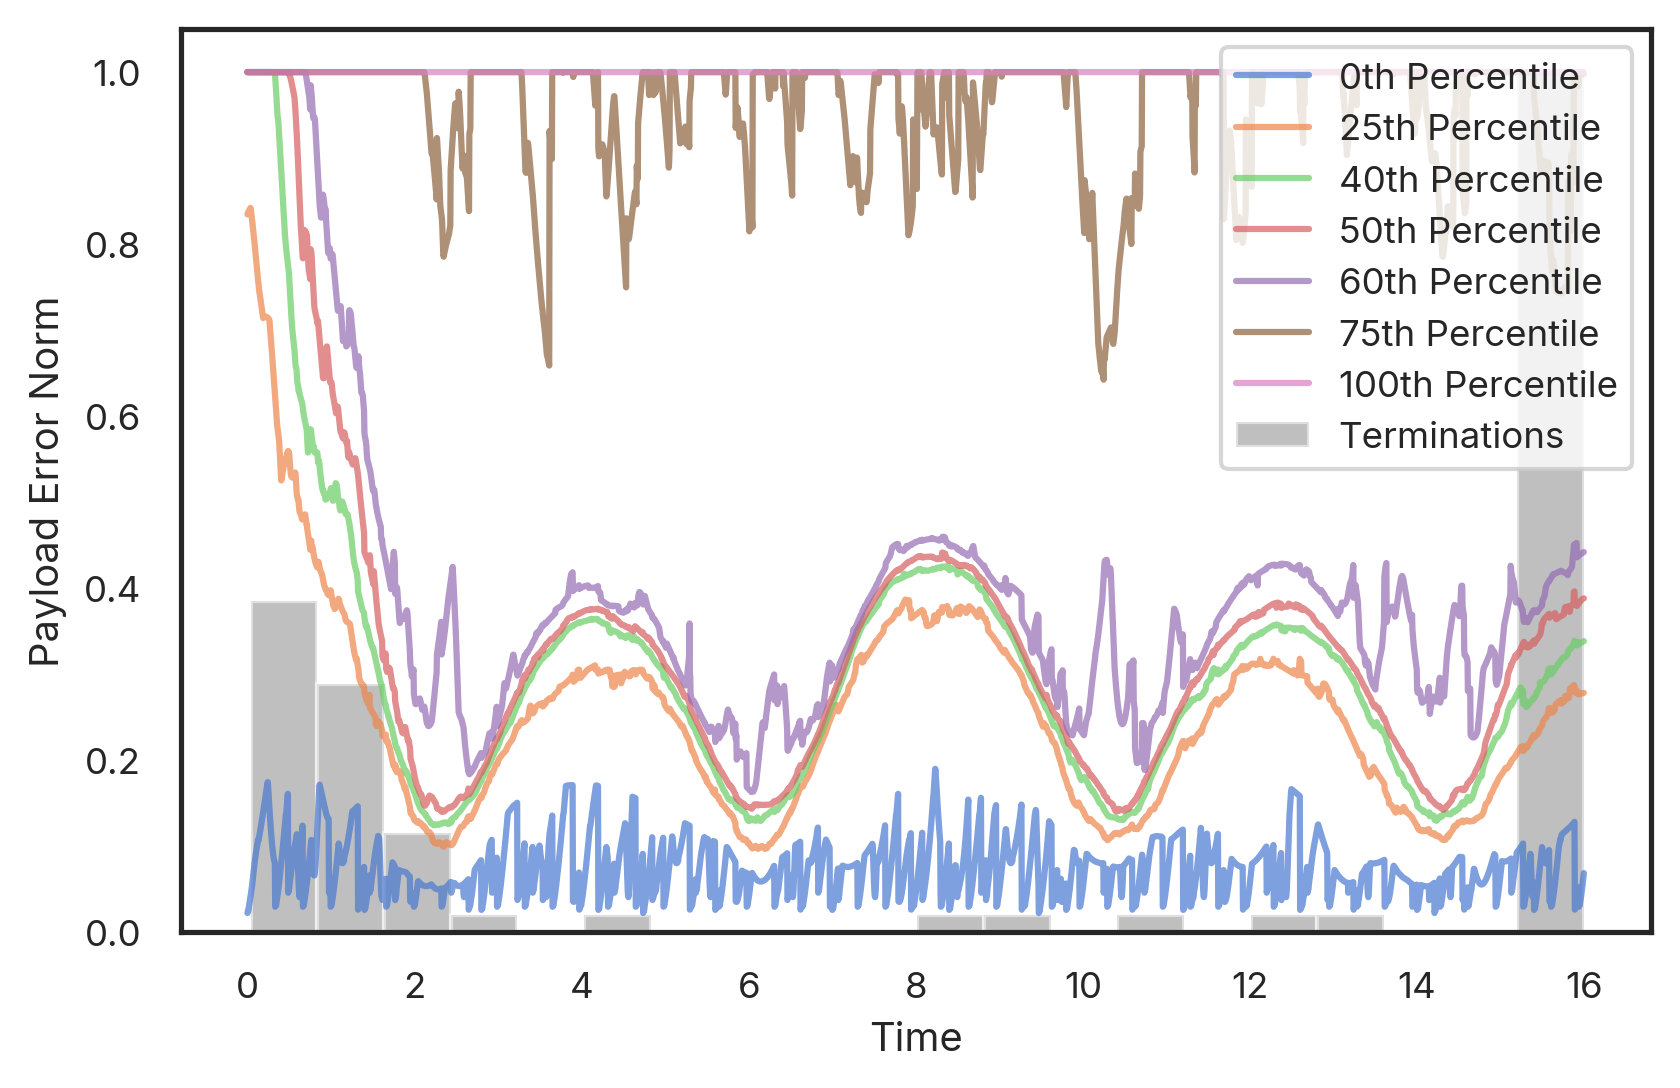
\includegraphics[width=\textwidth]{experiments/payload_error_over_time.png}
        \caption{Error over time for 3 quadrotors with payload (1000 rollouts).}
        \label{fig:payload_error_3quads}
    \end{subfigure}
    \hfill
    \begin{subfigure}[b]{0.49\textwidth}
        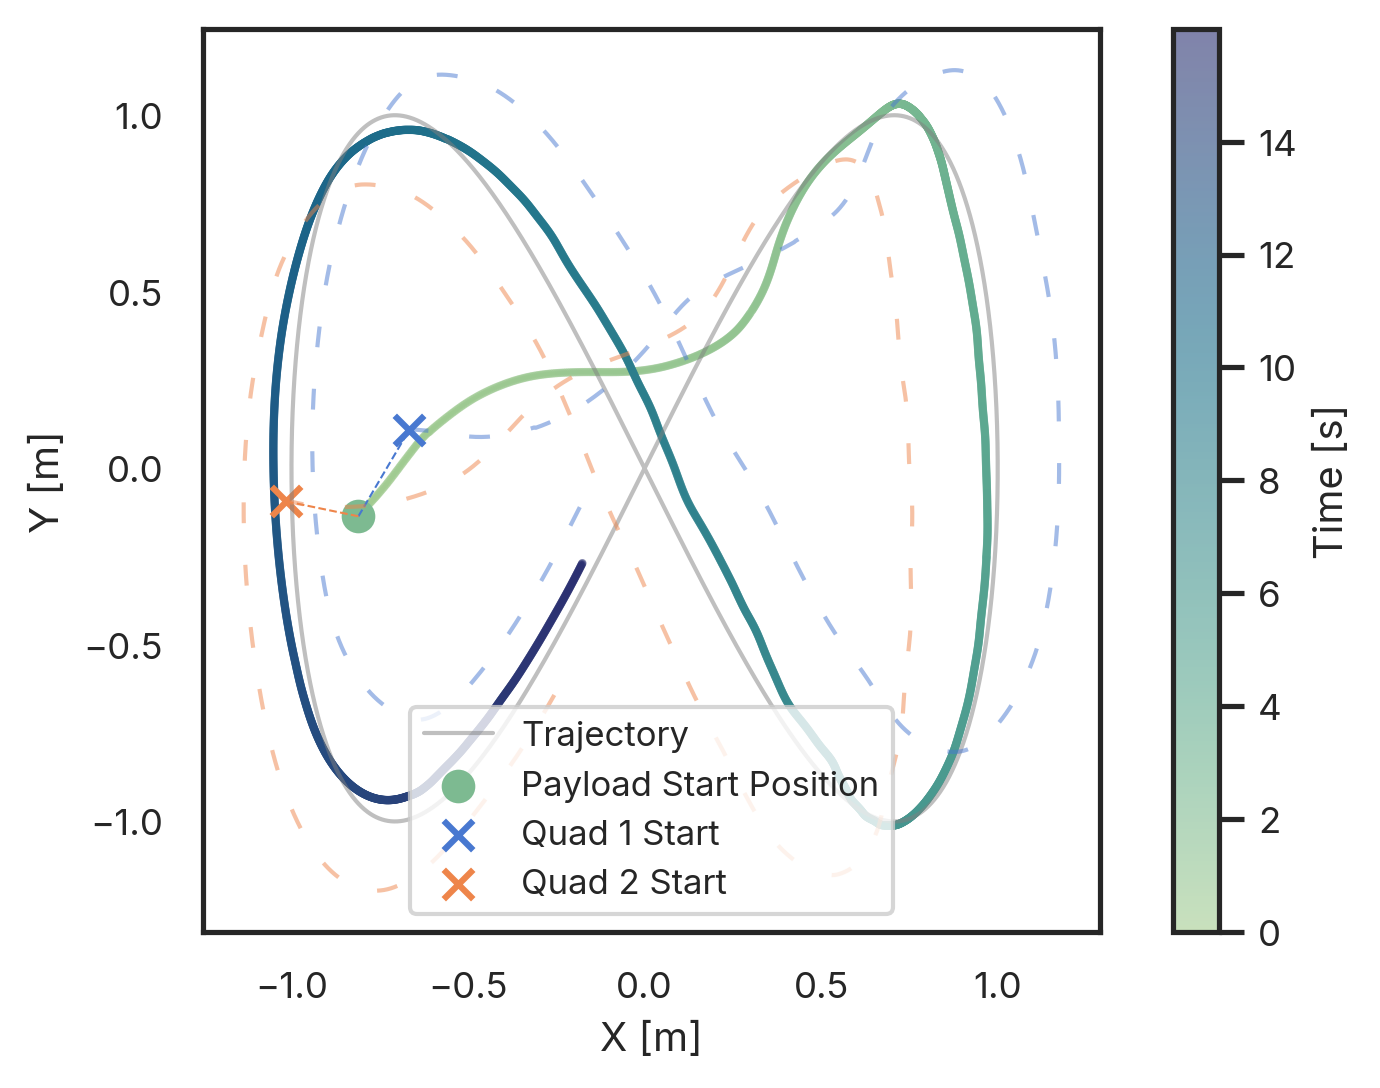
\includegraphics[width=\textwidth]{experiments/payload_position_xy.png}
        \caption{Position tracking for 3 quadrotors on figure-eight.}
        \label{fig:payload_position_3quads}
    \end{subfigure}

    \vspace{1em}

    % Five quadrotors
    \begin{subfigure}[b]{0.49\textwidth}
        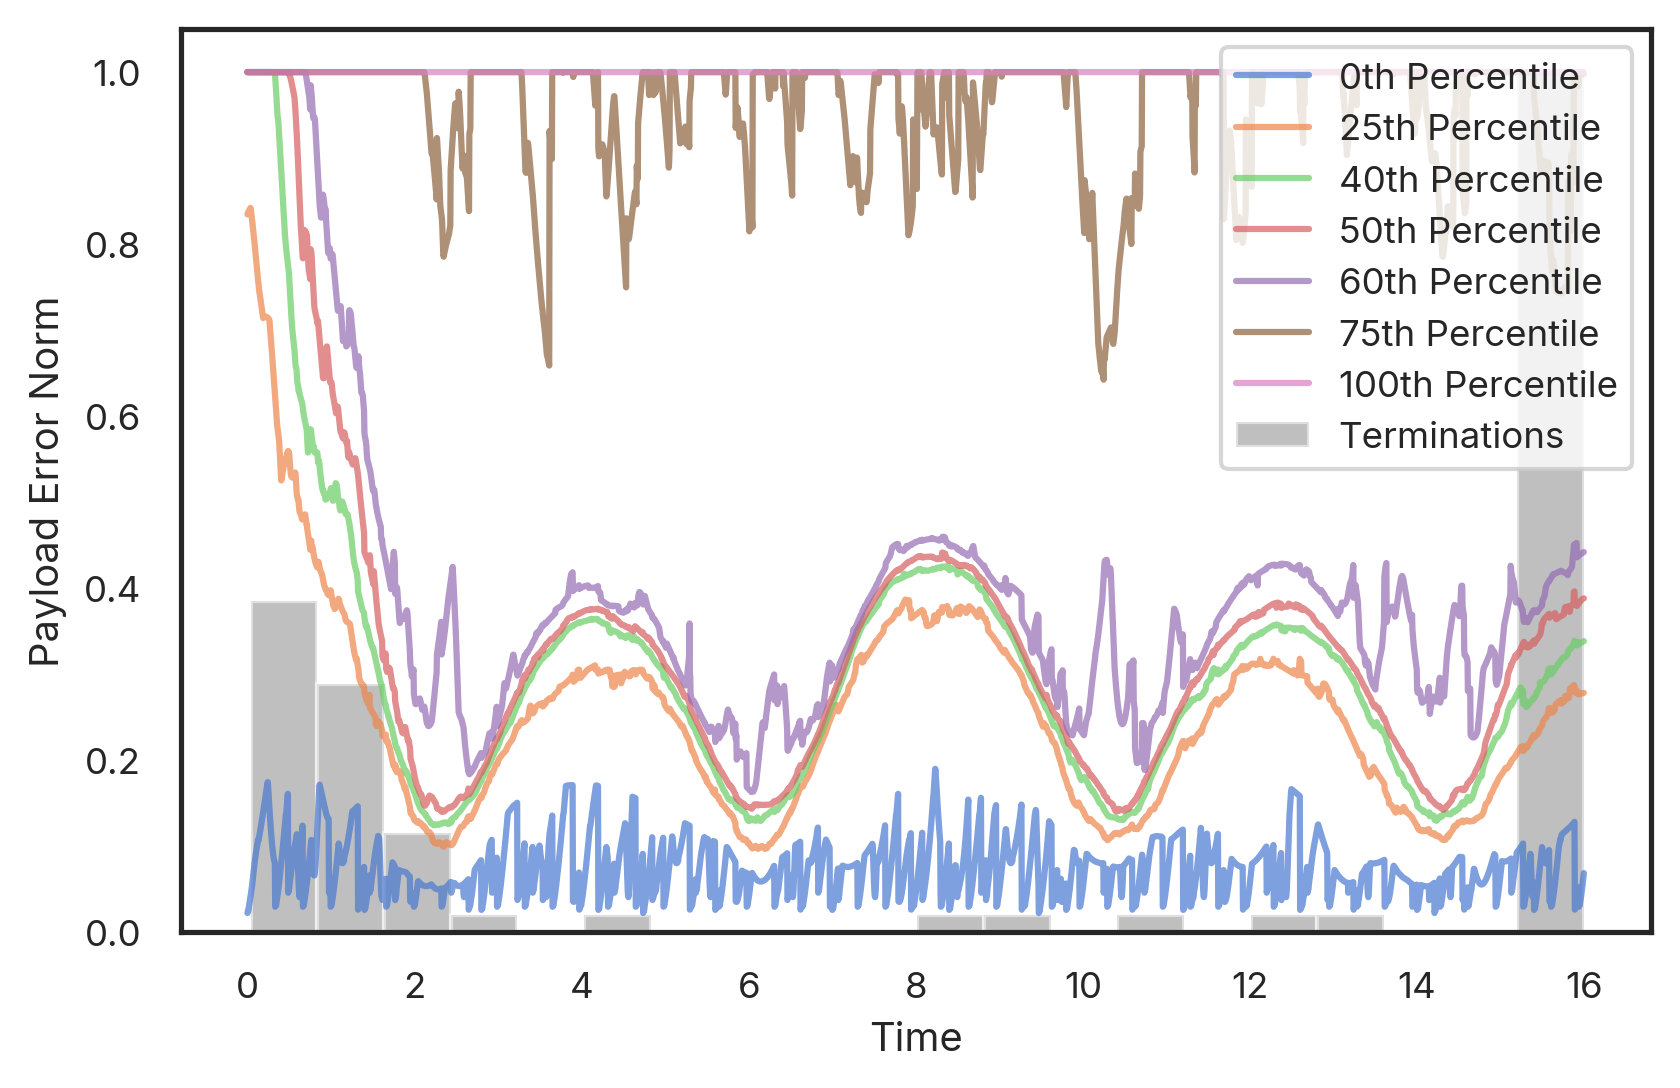
\includegraphics[width=\textwidth]{experiments/payload_error_over_time.png}
        \caption{Error over time for 5 quadrotors with payload (1000 rollouts).}
        \label{fig:payload_error_5quads}
    \end{subfigure}
    \hfill
    \begin{subfigure}[b]{0.49\textwidth}
        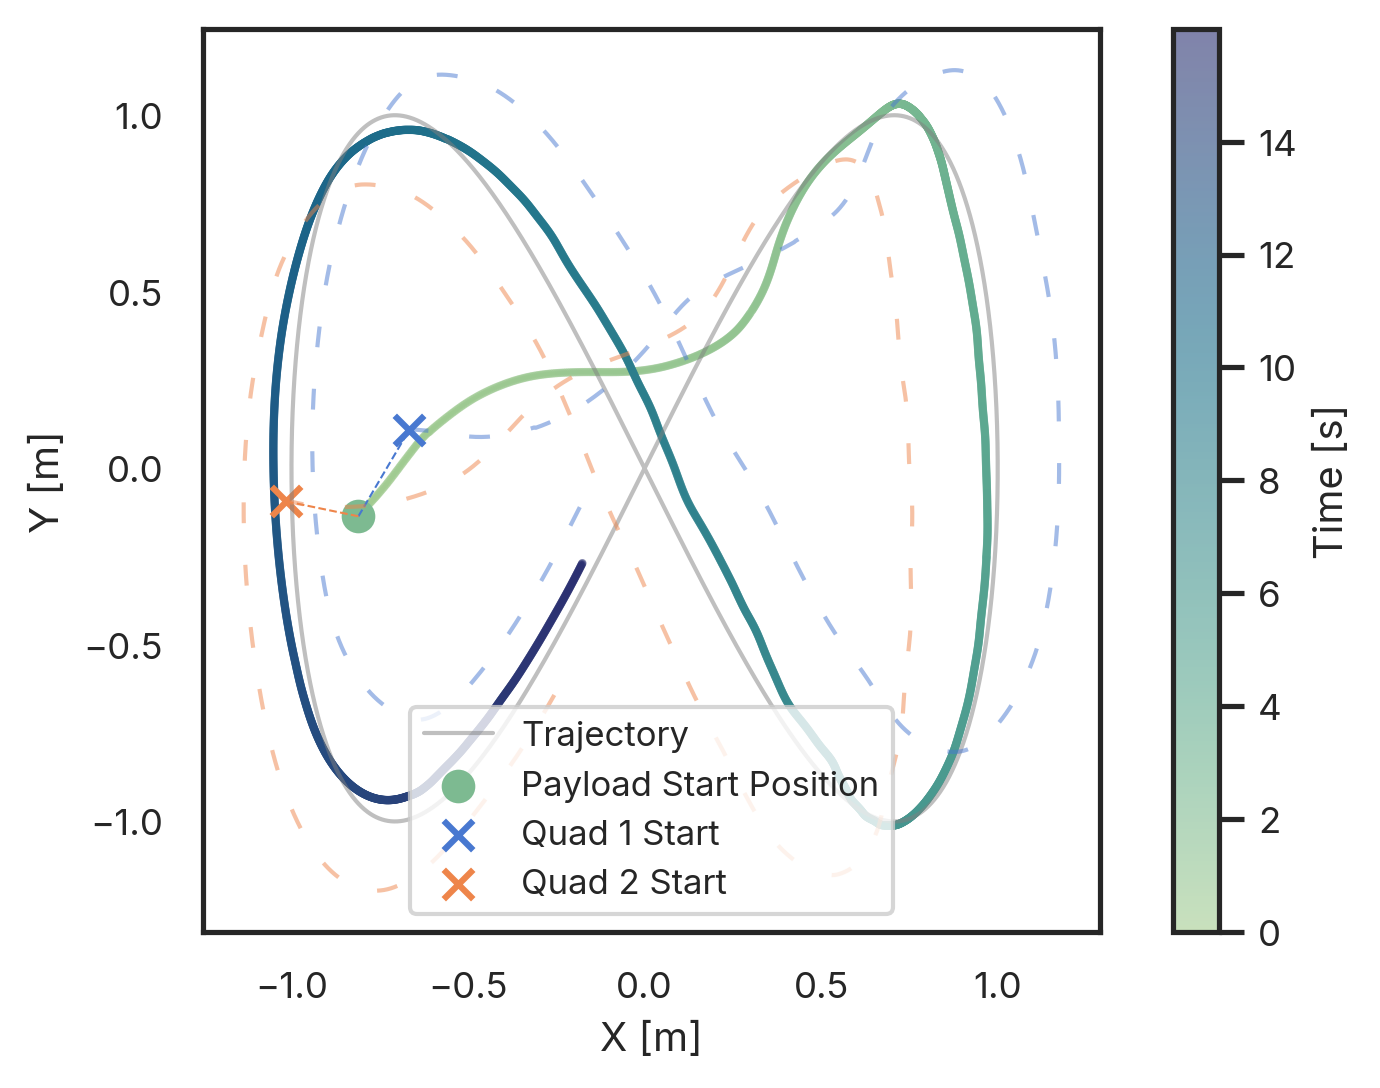
\includegraphics[width=\textwidth]{experiments/payload_position_xy.png}
        \caption{Position tracking for 5 quadrotors on figure-eight.}
        \label{fig:payload_position_5quads}
    \end{subfigure}

    \caption{Multi-quadrotor control with payload: rows correspond to 2, 3, and 5 quadrotors. (a),(c),(e) error over time; (b),(d),(f) position tracking.}
    \label{fig:multi_quad_payload}
\end{figure}
\begin{itemize}
    \item Recover from harsh and track position
    \item Follow trajectory
    \item Follow trajectory with disturbance
    \item Plots recovery: Recovery success rate for 10000 rollouts ofver time.
    \item Plots Traj: Trajectory following 3d, error over time for batch
    \item Plots Disturbance: Trajectory following with disturbance, error over time for batch
\end{itemize}
% optional
\section{Comparison with classic control}
Compare with prev paper method \autocite{Wahba2024}
\begin{itemize}
    \item Plots Traj: Trajectory following 3d, error over time for batch
    \item Plots Disturbance: Trajectory following with disturbance, error over time for batch
    \item Plots ground start: Trajectory following with disturbance, error over time for batch
\end{itemize} 
\section{Sim-to-Real Transfer}
\begin{itemize}
    \item one and three quads
    \item Plots Traj: Trajectory following 3d,  error over time 
    \item Plots Disturbance: Position holding with disturbance
\end{itemize}


\section{Ablation Studies}
\begin{itemize}
    \item Ablation on reward design
    \item Ablation on training parameters
    \item Ablation on domain randomization
    
\end{itemize}